\subsection{Research Objectives and Anticipated Results}

%\begin{wrapfigure}{l}{0.62\textwidth}
%\begin{figure}[t]
%    \centering
%    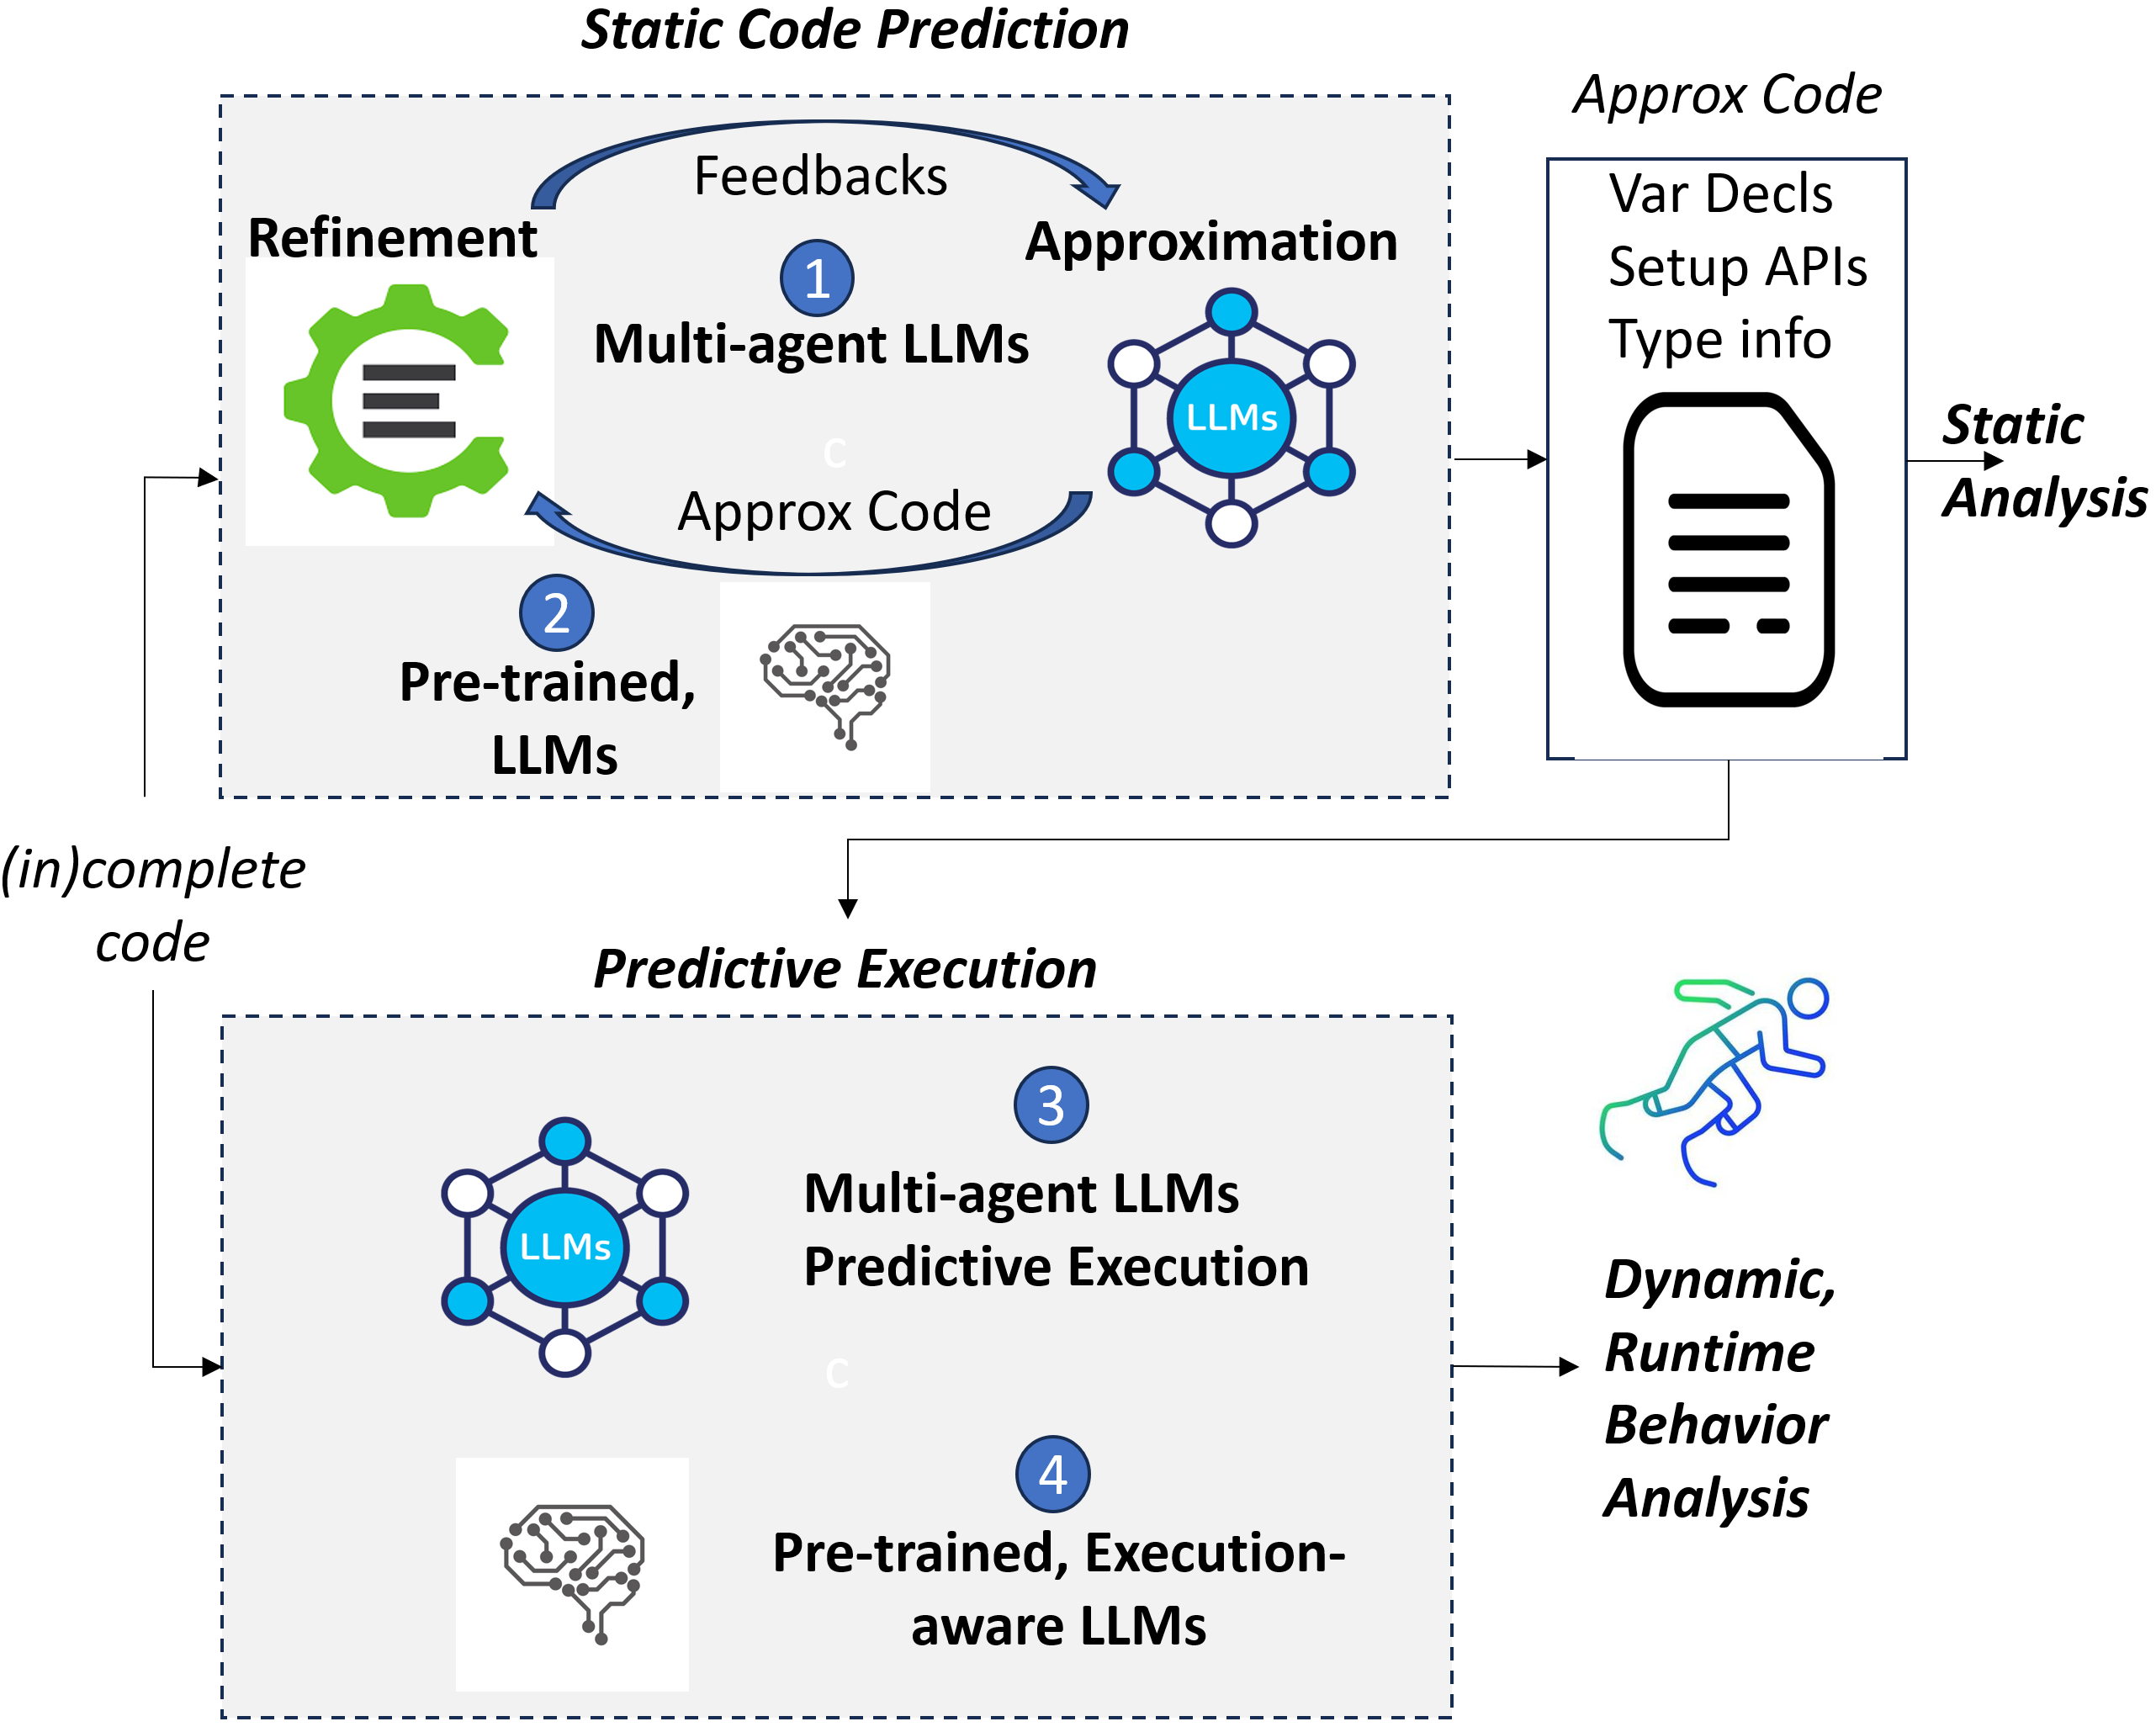
\includegraphics[width=0.62\textwidth]{overview-new.png}
%    \vspace{-10pt}
%    \caption{Predictive Program Analysis: Analyzing Dynamic Program Behaviors}
%    \label{fig:arch}
%\end{wrapfigure}


We seek to advance the state-of-the-art in fuzz testing by means of
{\tool}, a {\bf Predictive Coverage-Guided Intelligent Fuzzing}
framework, with the goal of overcoming the issues listed in the
introduction. We aim to establish {\em a scientific foundation, novel
  methodologies, frameworks, models, and algorithmic solutions for
  predictive coverage-guided fuzz testing} with the following focus
areas:



(1) Large Language Models (LLM)-based {\bf predictive code coverage} (without test execution),

(2) LLM-based, targeting, {\bf test case generation}, and

(3) {\bf predictive coverage-guided fuzz testing} with LLMs.

%\noindent Figure~\ref{fig:arch} illustrates the framework for {\tool},
%which will allow the construction of efficient program analysis
%techniques for (partial) code, also based on which downstream vulnerability detection and assessment applications can be built.

Our predictive program analysis framework is also beneficial in other
scenarios in addition to programming assistants for incomplete code in
an IDE. Predictive execution is not aimed to replace actual
execution. Rather, it offers a solution where the actual execution is
impossible, specifically in the scenarios 1) where the complete source
code is not available, or 2) where the analysis or approximation on
the behavior of the code is needed/desired without actual execution
and some degree of inaccuracy in prediction is tolerable.  First, the
first scenario can be exhibited in several examples, e.g., in the code
snippets in Stack Overflow or GitHub gist. They often miss contextual
information, such as imports and definitions of variables and
functions. It can take a great deal of efforts to integrate such code
snippets to a codebase.
%Horton and Parnin~\cite{horton2018gistable} reported that ``75.6\% of
%Python code snippets in gist require non-trivial configuration to
%overcome missing dependencies, configuration files, reliance on a
%specific operating system, or some other environment
%configuration''. Hossain {\em et al}~\cite{hossain2019executability}
%found that after installing the top 40~Python packages, the overall
%execution success rate for Stack Overflow Python code snippets is only
%27.9\% considering those running in either Python 2 or Python 3
%environments.
%Moreover, in~his keynote,
%Yahav~\cite{yahav2023fse} poses a need to approximate the execution of
%the incomplete code under editing in an AI-assisted programming
%environment.
Second, the instances of the second scenario can include the
analysis/approximation~of the behavior to check properties of
untrusted code or~to~detect bugs early. Moreover, even with complete
code, setting~up running environments for dynamic analysis is
undesired due to missing third-party dependencies and complex build
configurations.

The \underline{key philosophy} that drives our work is that the analysis of
partial code can be learned from the analysis of entire programs in
the wealth of information obtained from ultra-large-scale, open-source
software repositories. To accomplish these tasks, we propose the
following thrusts of research in {\tool}:

\noindent \textbf{Thrust 1. LLM Multi-agents and Pre-trained Language Models for Static Analysis on Incomplete Code.} ({\em Section~\ref{sec:thrust1}})



%As depicted in Figure~\ref{fig:pre-rec}, conventional Program Analysis (PA) techniques exhibit high precision and recall when applied to complete code. However, when dealing with incomplete code, these techniques may experience a significant decrease in recall due to missing information, despite maintaining reasonably high precision or experiencing a slight decrease in precision due to their strict and/or heuristic analysis rules (denoted by PA $\medblacklozenge$ in Figure~\ref{fig:pre-rec}). On the other hand, employing an LLM directly for downstream analysis tasks may yield higher recall, thanks to the LLM's ability to explore the solution space (denoted by LLM $\circledast$ in Figure~\ref{fig:pre-rec}). However, the precision of   LLM analysis on incomplete code tends to be lower compared to conventional PA tools due to the lack of ability in specific analysis in the downstream tasks.

%We propose a tandem solution that combines LLMs and PA agents to
%leverage the strengths of both methodologies. We aim to harnessing the
%complementary capabilities of LLMs and PA: {\em LLMs' expansive search
%  capabilities} and {\em PA-based agents' semantic verification
%  abilities}.

%We advocate for a novel paradigm, called {\bf predictive program
%  analysis}, which operates on the principles of {\em
%  Approximation-Refinement} for Analysis. In the Approximation phase,
%a large language model (LLM) acts as a machine learning (ML) agent to
%fill in missing information within incomplete code. The missing
%information that will be filled by the LLM could be manifested {\em
%  explicitly}, e.g., in terms of missing variable declarations, setup
%API method calls, import statements, and exception handling types, or
%{\em implicitly}, e.g., in terms of missing type information of 
%program elements, missing dependencies, etc.

%\begin{wrapfigure}{l}{0.55\textwidth}
    \centering
    \begin{tikzpicture}
        \pgfplotsset{width=3in,
         }
        \begin{axis}[
            scale=1,
            view={20}{35},
            ticklabel style={font=\footnotesize},
            xlabel={\normalsize \textbf{Precision} ($\rightarrow$)},
            ylabel={\normalsize \textbf{Recall} ($\rightarrow$)},
%            zlabel={\normalsize \textbf{Source Code} ($\rightarrow$)},
            xlabel style={rotate=-10, yshift=0.1cm},
            ylabel style={yshift=0.5cm, xshift=0.225cm,rotate=65},
            zlabel style={yshift=-0.2cm, xshift=-0.5cm,rotate=0},
            xmin=0, xmax=4,
            xtick={1,2,3},
            ymin=0, ymax=4,
            ytick={1,2,3},
            zmin=0, zmax=1,
            ztick={0,1},
            xticklabels={\textit{Low},\textit{Medium},\textit{High}}, % Set custom x-tick labels
            yticklabels={\textit{Low},\textit{Medium},\textit{High}}, % Set custom y-tick labels
            zticklabels={\textit{Partial Code},\textit{Complete Code}},
            ztick pos = left,
            xticklabel style={rotate=0},
            yticklabel style={rotate=0, yshift=0.325cm},
            zticklabel style={yshift=0.4cm},
            % Set custom z-tick labels
            axis background/.style={fill=gray!10},
            xmajorgrids=true,
            ymajorgrids=true,
            zmajorgrids=true,
            grid style={dotted, thick},
            axis equal,
            visualization depends on={value \thisrow{m} \as \labela},
        ]
        % Add a node at x=High, y=High, z=Complete
        \draw[dashed,black,thick] (axis cs:3,3,1) -- (axis cs:0,3,1) node[midway, right] {};
        \draw[dashed,black,thick] (axis cs:3,3,1) -- (axis cs:3,4,1) node[midway, below] {};
        \draw[dashed,black,thick] (axis cs:3,3,1) -- (axis cs:3,3,-0.2);
        \node[above right] at (axis cs:{2.9,2.55,1}) {\textcolor{blue}{\large $\medblacklozenge$}};

        % Thick axes
        \draw[black, thick] (axis cs:0,4,-0.3) -- (axis cs:4,4,-0.3) node[midway, right] {};
        \draw[black, thick] (axis cs:0,4,-0.3) -- (axis cs:0,0,-0.3) node[midway, right] {};
        \draw[black, thick] (axis cs:0,4,-0.3) -- (axis cs:0,4,1.3) node[midway, right] {};
        

        % Add points.
        \node[above right] at (axis cs:{3,0.75,0}) {\textcolor{red}{\large $\medblacklozenge$}};
        \node[above right] at (axis cs:{2.95,1.85,0}) {{\textcolor{meatbrown}{\small $\bigstar$}}};
        \node[above right] at (axis cs:{2.55,1.5,0}) {\textcolor{red}{{\small $\circledast$}}};

        % % Add Origin
        % \node[above right] at (axis cs:{4,-0.2,0}) { $\circ$};

        % Add optimal point
        \node[above right] at (axis cs:{3.08,2.3,0}) { \textcolor{dkgreen}{{\footnotesize $\circ$}}};

        \end{axis}
        \draw[gray,line width=0.5pt,rotate=15,fill=red,opacity=0.125] (3.75,0.85,0) circle (1.75 and 0.85);

        % Add node labels
        \node[text width=2cm] at (6,3.75,1) 
            {\footnotesize{\textcolor{blue}{PA}}};
        \node[text width=2cm] at (5.0,1.275,0) 
            {\footnotesize{\textcolor{red}{PA}}};
        \node[text width=2cm] at (4,2.025,0) 
            {\footnotesize{\textcolor{red}{LLM+PA}}};
         \node[text width=2cm] at (3.875,1.7,0) 
            {\footnotesize{\textcolor{red}{LLM}}};
    \end{tikzpicture}
    \vspace{-20pt}
    \caption{Efficacy of various \textcolor{red}{\textit{\textbf{partial}}} and \textcolor{blue}{\textit{\textbf{complete}}} program analysis approaches, with ({\small $\medblacklozenge$}), and without ({\footnotesize $\circledast$}, {\footnotesize $\bigstar$}) learning-based knowledge.}
    \label{fig:pre-rec}
\end{wrapfigure}


%A naive solution is to take whatever information the LLMs completed
%and feed to a traditional program analysis as is. However,
%researchers have shown that while LLMs are remarkable in code
%generation with correct syntaxes, the produced code often contains
%semantic errors and even do not compilable.  Thus, the Refinement
%phase employs a program analysis (PA)-based agent to verify the
%completed code output by the LLM. This PA-based agent utilizes the
%compiler technology to ensure that the generated code is compilable
%and consistent with used external libraries. The iterative interplay
%between the LLM-based agent and the PA-based agent continues until a
%compilable code is achieved.
%In brief, the interplay between LLM and PA agents has two objectives:
%1) to enhance recall compared to the PA-only solution (via the
%Approximation of the incomplete code), and 2) to
%maintain or even improve precision beyond what can be achieved with
%LLM-only solution by integrating PA to ``correct'' the LLM's solution
%(via the result Refinement).

%While exploring LLM-based multi-agent solution, we also aim to develop
%smaller models via pre-trained language models. Our work is driven by
%the fundamental belief that insights gained from training by complete
%programs within vast repositories of ultra-large-scale, open-source
%software can inform the analysis of partial code~\cite{naturalness-icse12}.
%Thus, we expect to build/fine-tune pre-trained LLM models to learn
%from those repositories.

%\vspace{3pt}
%\noindent \textbf{Thrust 2. LLM Multi-agents and Pre-trained
%  Language Models for Predictive Execution.}  ({\em
%  Section~\ref{sec:thrust2}})

%We advocate for an execution paradigm called predictive execution. In
%predictive execution, with a specific input, the execution is not
%carried out with the computer performing the instruction in the
%program. Instead, a trained machine learning model predicts the
%execution steps and as a result, the execution trace corresponding to
%the input is derived without actual execution.

%By simulating program behaviors and outcomes without running the code,
%these approaches provide valuable insights into the program's
%potential runtime characteristics. Here are some benefits of
%predictive execution. First, early error detection: predicting program
%executions allows for the early detection of errors and potential
%vulnerabilities before executing the code. By simulating different
%execution paths and scenarios, predictive execution can enable the
%dynamic analysis tools to identify potential issues such as null
%pointer dereferences, memory leaks, or buffer overflows without the
%need to execute the code in a real-world environment. This early error
%detection helps developers catch and fix bugs more efficiently,
%reducing the likelihood of critical issues in production. Second,
%dynamic analysis techniques that predict program executions play a
%crucial role in security analysis. By simulating potential attack
%scenarios and analyzing how the program behaves under different
%conditions, these tools can identify security vulnerabilities such as
%injection attacks, privilege escalation, or data breaches. Predictive
%execution helps security professionals assess the resilience
%of systems against various threats and vulnerabilities,
%enabling proactive security measures and robust defenses. Finally,
%predicting executions provides developers with a deeper understanding
%of their code's behavior without the need for actual execution. By
%simulating program flows and interactions, tools can uncover hidden
%dependencies, identify unexpected behaviors, and reveal complex
%program dynamics.

%In addition multi-agent solutions, we also explore the
%pre-training language models. We aim to teach a smaller model to analyze
%the runtime behaviors via the learning from complete programs in execution.

%\vspace{3pt}
%\noindent \textbf{Thrust 3. Programming Assistant Applications with Predictive Program Analysis.}  ({\em Section~\ref{sec:thrust3}})


%Our last thrust of research is aimed to demonstrate the usefulness of
%our solution in different programming assistant applications: 1)
%vulnerability detection, 2) dynamic slicing,  etc.

\begin{table*}[t]
	\vspace{-15pt}
\begin{center}
{\footnotesize{
\begin{tabular}{cc}
\begin{tabular}[t]{|p{0.2in}|p{2.95in}|} 
\hline
\multicolumn{2}{|>{\columncolor[gray]{0}}c|}{\textcolor{white}
{\bf Year 1 Project Milestones \& Deliverables}}\\
\hline 
\hline
\multicolumn{2}{|c|}{\bf T1. LLM Multi-agents for Static Analysis}\\
\hline
{\bf 1.1} & LLM Multi-agent framework\\
{\bf 1.2} & LLM Multi-agent and Static Analysis\\
{\bf 1.3} & Pre-trained Language Models for Static Analysis\\
\hline
\hline
\multicolumn{2}{|c|}{\bf T1. Pre-trained Language Models for Static Analysis}\\ 
\hline
{\bf 1.4} & Pre-trained Language Models for Static Analysis\\
\hline
%\hline
%\multicolumn{2}{|c|}{\bf Integrate Code Synthesis into Tools}\\
%\hline
%{\bf 1.5} & \goalOneFour.\\
%\hline
\multicolumn{2}{c}{}
\end{tabular}
&
\begin{tabular}[t]{|p{0.2in}|p{2.95in}|} \hline
\multicolumn{2}{|>{\columncolor[gray]{0}}c|}{\textcolor{white}
{\bf Year 2 Project Milestones \& Deliverables}}\\
\hline 
\hline
\multicolumn{2}{|c|}{\bf T2. LLM Multi-agents for Predictive Execution}\\
\hline
{\bf 2.1} & LLM Multi-agents with Graphs\\
{\bf 2.2} & LLM Multi-agents with Execution\\
%{\bf 2.3} & Integrate Evaluation Framework into Design Environment\\
%{\bf 2.4} & Evaluate CRL Framework with Existing Models\\
%{\bf 2.3} & \goalTwoThree.\\

\hline
\hline
\multicolumn{2}{|c|}{\bf T2. Pre-trained Language Models for Predictive Execution}\\ 
\hline
%{\bf 3.1} & Design New Code Representations and Learning Models.\\
{\bf 2.3} &  Pre-trained Language Models for Predictive Execution\\
%{\bf 2.4} & Advance FL and RT-CI Approaches.\\
%{\bf 2.5} & Advance Regression Testing in CI Approaches.\\
%{\bf 2.5} & Advance APR Approaches with Framework.\\
\hline
%\hline
%\multicolumn{2}{|c|}{\bf Community Involvement: Capacity Building}\\
%\hline
%{\bf 2.4} & \goalTwoFour.\\
%{\bf 2.5} & \goalTwoFive.\\
%{\bf 2.6} & \goalTwoSix.\\
%\hline
\multicolumn{2}{c}{}
\end{tabular}
\end{tabular}\\
\vspace*{-.3cm}
\begin{tabular}{c}\hline
\multicolumn{1}{|>{\centering\columncolor[gray]{0}}p{6.44in}|}{\textcolor{white}
{\bf Year 3 Project Milestones \& Deliverables}}\\
\hline
\end{tabular}\\
\vspace*{-.2cm}
\begin{tabular}{cc}
\begin{tabular}[t]{|p{0.2in}|p{2.95in}|}
\hline
\multicolumn{2}{|c|}{\bf T3. Programming Assistant with Predictive Analysis}\\
\hline
{\bf 3.1} & Dependency Analysis\\
{\bf 3.2} & Debugging and Error Detection\\
\hline
%\hline
%\multicolumn{2}{|c|}{\bf \goalTwo}\\ 
%\hline
%{\bf 3.3} & \goalThreeThree.\\
%\hline
\multicolumn{2}{c}{}
\end{tabular}
&
\begin{tabular}[t]{|p{0.2in}|p{2.95in}|}
\hline
\multicolumn{2}{|c|}{\bf T3. Programming Assistant with Predictive Analysis}\\
\hline
%{\bf 3.1} & Design New Code Representations\\
{\bf 3.3} & Dynamic Slicing\\
\hline
\multicolumn{2}{c}{}
\end{tabular}
\end{tabular}
\vspace{-15pt}
}}
\end{center}
\vspace*{-.3in}
%\caption{Tasks and Milestones. (Rep. = Representation)}
\caption{The 3-year schedule of Thrusts, Tasks, and Milestones of this proposal.}
%the schedule of Thrusts, Tasks, and Milestones of this proposal.
%\vspace{-10pt}
\label{tab:milestones}
\vspace{-10pt}
\end{table*}
%

